\section{Filtering}
\label{sec:filtering}

\begin{figure}[H]
  \center
    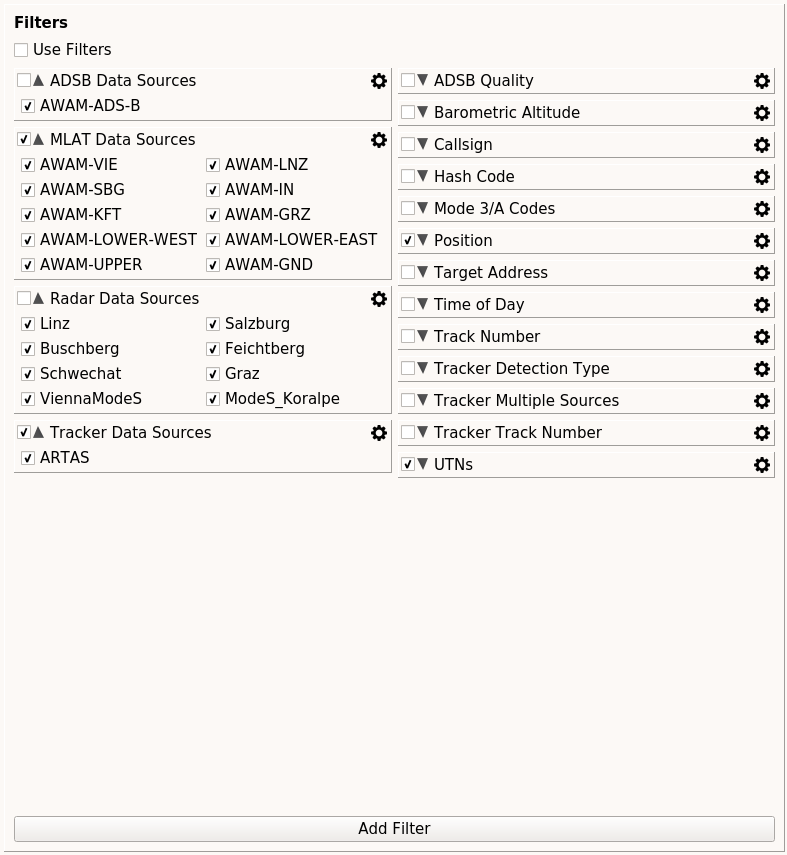
\includegraphics[width=14cm,frame]{../screenshots/load_filters.png}
  \caption{Default filters}
\end{figure}

\subsection{Data Source Filters}

\begin{figure}[H]
  \center
    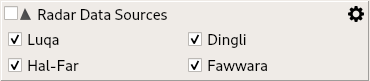
\includegraphics[width=8cm,frame]{../screenshots/filter_datasources.png}
  \caption{Data Sources filter}
\end{figure}

Multiple of these filters can exist, depending on which DBObjects exist in the database. \\

When active, each of these filters forces loading of data only from the selected data sources. \\

\subsection{Barometric Altitude Filter}

\begin{figure}[H]
  \center
    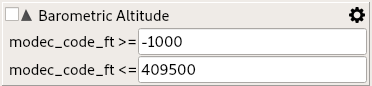
\includegraphics[width=8cm,frame]{../screenshots/filter_baro_alt.png}
  \caption{Barometric Altitude filter}
\end{figure}

When active, this filter forces loading of data with a barometric altitude inside the given thresholds (in feet). Target reports without a barometric altitude will not be loaded.

\subsection{Callsign Filter}

\begin{figure}[H]
  \center
    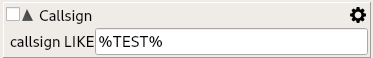
\includegraphics[width=8cm,frame]{../screenshots/filter_callsign.png}
  \caption{Callsign filter}
\end{figure}

When active, this filter forces loading of data only from callsigns matching the given expression. The percent operator denotes a 'any characters' placeholder. So e.g. '\%TEST\%' will match 'TEST123' or 'TEST123   ' (with spaces) or 'MYTEST'. Target reports without a given callsign will not be loaded.

\subsection{Hash Code Filter}

\begin{figure}[H]
  \center
    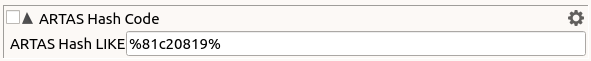
\includegraphics[width=8cm,frame]{../screenshots/filter_hashcode.png}
  \caption{Hash Code filter}
\end{figure}

When active, this filter forces loading of data only from target reports with a specific ARTAS MD5 hash code, or system track updates referencing this hash code (in their TRI information). If no hash information is available (e.g. in SASS-C Verif databases or when this information was not present in the ASTERIX data), this filter should not be used.

\subsection{Mode 3/A Code Filter}

\begin{figure}[H]
  \center
    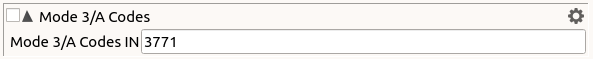
\includegraphics[width=8cm,frame]{../screenshots/filter_mode3a.png}
  \caption{Mode 3/A Code filter}
\end{figure}

When active, this filter forces loading of data with the given Mode A code(s), so it is possible to give multiple values (in octal notation, separated by commas). E.g. '7000' is possible, or '7000,7777'. Target reports without a given Mode A will not be loaded unless the value 'NULL' is (also) given. \\

Please note that ADS-B target reports can also contain Mode 3/A code information.

\subsection{Position Filter}

\begin{figure}[H]
  \center
    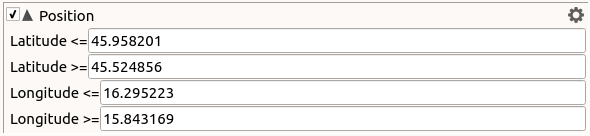
\includegraphics[width=8cm,frame]{../screenshots/filter_position.png}
  \caption{Position filter}
\end{figure}

When active, this filter forces loading of data with latitude/longitude inside the given thresholds (in degrees).

\subsection{Target Address Filter}

\begin{figure}[H]
  \center
    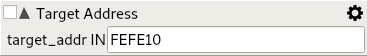
\includegraphics[width=8cm,frame]{../screenshots/filter_targetaddress.png}
  \caption{Target Address filter}
\end{figure}

When active, this filter forces loading of data with the given Mode S address(es), so it is possible to give multiple values (in hexadecimal notation, irrespective of upper or lower case characters, separated by commas). E.g. 'FEFE10' is possible, or 'FEFE10,FEFE11,FEFE12'. Target reports without a given Mode S address will not be loaded unless the value 'NULL' is (also) given.

\subsection{Time of Day Filter}

\begin{figure}[H]
  \center
    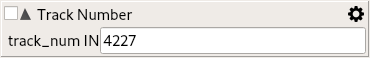
\includegraphics[width=8cm,frame]{../screenshots/filter_tod.png}
  \caption{Time of Day filter}
\end{figure}

When active, this filter forces loading of data with the time-of-day inside the given thresholds (in HH:MM:SS.SSS).

\subsection{Track Number Filter}

\begin{figure}[H]
  \center
    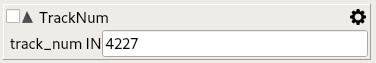
\includegraphics[width=8cm,frame]{../screenshots/filter_tracknum.png}
  \caption{Track Number filter}
\end{figure}

When active, this filter forces loading of data with the given track numbers, so it is possible to give multiple values (separated by commas). E.g. '1' is possible, or '1,2,3'. Target reports without a given track number will not be loaded unless the value 'NULL' is (also) given. \\

Please note that ADS-B target reports can also contain a track number in ASTERIX, but since the information can not currently be mapped to the database (missing in schema), this filter does not influence ADS-B data loading.

\subsection{Tracker Detection Type Filter}

\begin{figure}[H]
  \center
    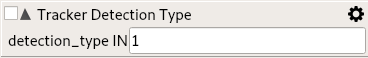
\includegraphics[width=8cm,frame]{../screenshots/filter_trackerdettyp.png}
  \caption{Tracker Detection Type filter}
\end{figure}

When active, this filter forces loading of Tracker data with the given detection type, so it is possible to give multiple values (separated by commas). E.g. '1' is possible, or '1,2,3'. Tracker target reports without a given detection type will not be loaded. \\

The following detection types exist:
\begin{itemize}
 \item 0: No detection/unknown
 \item 1: PSR
 \item 2: SSR
 \item 3: Combined (PSR+SSR)
 \item 5: Mode S
 \item 7: Mode S Combined (PSR+Mode S)
\end{itemize}
\  \\

Please note that:
\begin{itemize}
 \item The detection type here reflects the technology used to update the track. E.g. an MLAT SSR detection + a PSR detection can form detection type 3 (Combined).
 \item The method used to determine the detection type is slightly different than in Verif
 \item The method used to determine the detection type is currently being discussed/tested by users and will be documented after being accepted.
\end{itemize}

\subsection{Tracker Multiple Sources Filter}

\begin{figure}[H]
  \center
    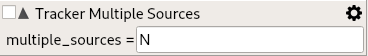
\includegraphics[width=8cm,frame]{../screenshots/filter_trackermulsrc.png}
  \caption{Tracker Multiple Sources filter}
\end{figure}

When active, this filter forces loading of Tracker data with the multiple sources flag, e.g. 'Y' (only track updates formed from multiple sources) or 'N' (only track updates formed using 1 source). Tracker target reports without such information will not be loaded.

\subsection{Tracker Track Number Filter}

\begin{figure}[H]
  \center
    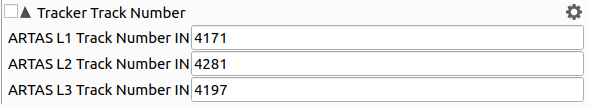
\includegraphics[width=8cm,frame]{../screenshots/filter_trackertracknum.png}
  \caption{Tracker Track Number filter}
\end{figure}

This filter works similiar to the 'Track Number' filter, but filters only DBObject Tracker, and allows for track numbers specific for each data source. E.g. '1' is possible, or '1,2,3', or '*' (all tracks).\\

It can be used when e.g. several Tracker runs were added, so that track numbers (from the same target) for each run can be specified seperately. \\

\subsection{UTN Filter}

\begin{figure}[H]
  \center
    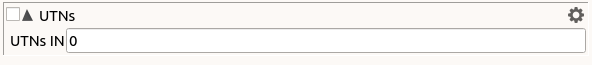
\includegraphics[width=8cm,frame]{../screenshots/filter_utn.png}
  \caption{UTN filter}
\end{figure}

This filter is only available if target report associations have been generated (see \nameref{sec:task_associate_tr}). \\

When active, this filter forces loading of data with the given unique target numbers (UTNs), so it is possible to give multiple values (separated by commas). E.g. '1' is possible, or '1,2,3'. Target reports without an associated UTN will not be loaded. \\

\subsection{Adding a New Filter}
When clicking the 'Add filter' button, a dialog is opened.

\begin{figure}[H]
  \center
    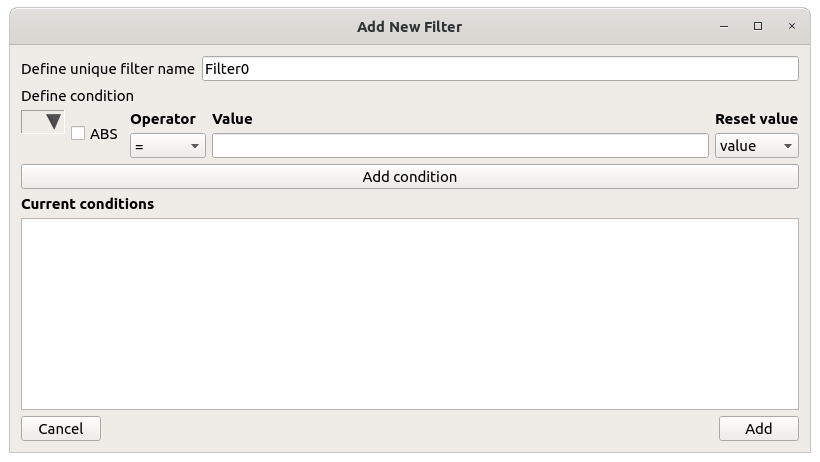
\includegraphics[width=14cm,frame]{../screenshots/filter_add.png}
  \caption{Adding a filter}
  \label{fig:filter_add}
\end{figure}

First, one has to give the filter a new (unique) name. Then, conditions have to be defined and added. A condition consists of a DBO variable, an operator, a value, and a reset value. \\

When the triangular button is clicked, a sub-menu is opened, where one can choose a DBO variable. The selected variable restricts data of all DBOs if it is of type 'Meta', or just data from one DBO if it is not.Additionally, the mathematical operator 'ABS' can be selected. If so, not the value of the variable but the absolute value of the variable is used: 'ABS(var)>value' is equivalent to 'var>value OR var<-value'. \\

An operator can be chosen with the drop-down menu, the supplied operators are common SQL operators.

\begin{table}[H]
  \center
  \begin{tabular}{ | l | l |}
    \hline
    \textbf{Operator} & \textbf{Description} \\ \hline
    = & Equal \\ \hline
    != & Not equal \\ \hline
    > & Greater than \\ \hline
    >= & Greater than or equal \\ \hline
    < & Less than \\ \hline
    <= & Less than or equal \\ \hline
    IN & Matches a value in a comma-separated list \\ \hline
    LIKE & Pattern matching with \% and \_ \\ \hline
    IS & Value NULL: No value exists \\ \hline
    IS NOT & Value NULL: Value exists \\
    \hline
  \end{tabular}
  \caption{SQL operators}
\end{table}

In the 'Value' field one can set a value manually, or load the minimum or maximum values of the selected DBO variable from the database using the 'Load min'/'Load max' buttons . A reset value also has to be supplied, which can be the chosen value or a minimum/maximum value set from the database.  Whenever a database different from the previous one is opened, all filters are reset, since previous values may have become invalid.\\

After a condition is defined, it has to be added using the 'Add condition' button. Existing conditions are shown in the 'Current conditions' list. Please note that for now added conditions can not be removed.

\begin{figure}[H]
  \center
    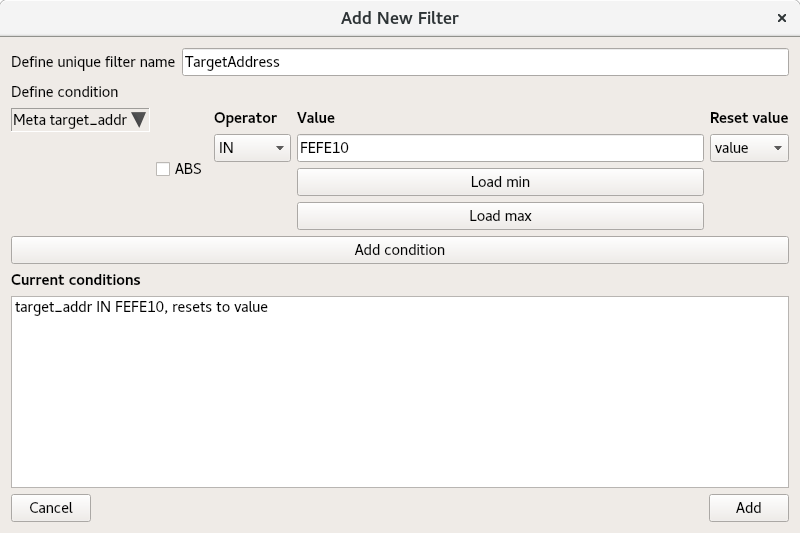
\includegraphics[width=14cm,frame]{../screenshots/filter_add2.png}
  \caption{Filled out filter dialog}
  \label{fig:filter_add2}
\end{figure}

Now the described process can be repeated until a usable filter emerges, which is added using the 'Add'
button. The process of adding a new filter can be canceled by using the 'Cancel' button, which discards all
settings. When added, a new filter shows up immediately in the filter list and is saved to the configuration
for persistence.

\begin{figure}[H]
  \center
    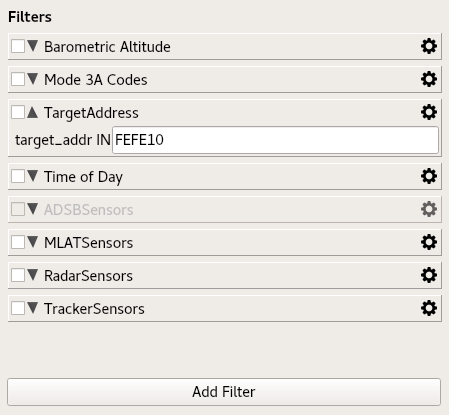
\includegraphics[width=8cm,frame]{../screenshots/filter_add3.png}
  \caption{Filter added}
  \label{fig:filter_add3}
\end{figure}

\subsection{Managing Filters}
\label{sec:filter_management}

By clicking on the gear symbol \includegraphics[scale=0.025]{../../data/icons/edit.png}, a menu allows the following operations on some of the filters:

\begin{itemize}  
\item Reset: Resets the filter to its default values.
\item Edit: Has been disabled and will be added at a later version.
\item Delete: Deletes a filter and permanently removes it from the configuration.
\end{itemize}
 
